%%==================================================
%% chapter01.tex for SJTU Master Thesis
%%==================================================

\chapter{Introduction}

\section{Motivation and Problem Description}
% motivation
With the spread of mobile devices, our life are crowded with many multimedia resources. 
Today, hundreds of millions pictures are being take, videos are uploaded, and a large amount of audio clips are also being recorded. 
Among these multimedia resources, audio data often contains many useful information around the device. 
For example, in an audio recorded under the context of office, we may hear "computer keyboard typing" and "phone ringing", sometimes with "people talking" as the background sound. 
After hearing these sound features, we human could easily deduce that the clips we heard are recorded in an office-like context. 
But this scene recognition process could be further speed up or applied to large quantity audios by a automatically scene recognition system.  

The automatical recognition for audio scenes are important for audio content analysis. 
For example, in the modern life, people tend to carry their mobile phones everywhere with them. 
It would be more convinient if the mobile devices could automatically adjust their volume and other profile settings according to the surrounding environment. 
This may prevent the trouble of unexpected loud noise by mobile devices in an quiet scene, or could save us from missing important notifications when we are surrounded by noisy atmosphere.  
Moreover, this technique not only could be applied in ordinary conditions, but also in some security issues. 
In the surveillance process, police may receive hundreds of thousands videos and audio clips. 
The automatic scene recognition technique may help to them fast analyze those audios and pindown the scenes they want to further analyze. 

\begin{figure}[htb]
\centering
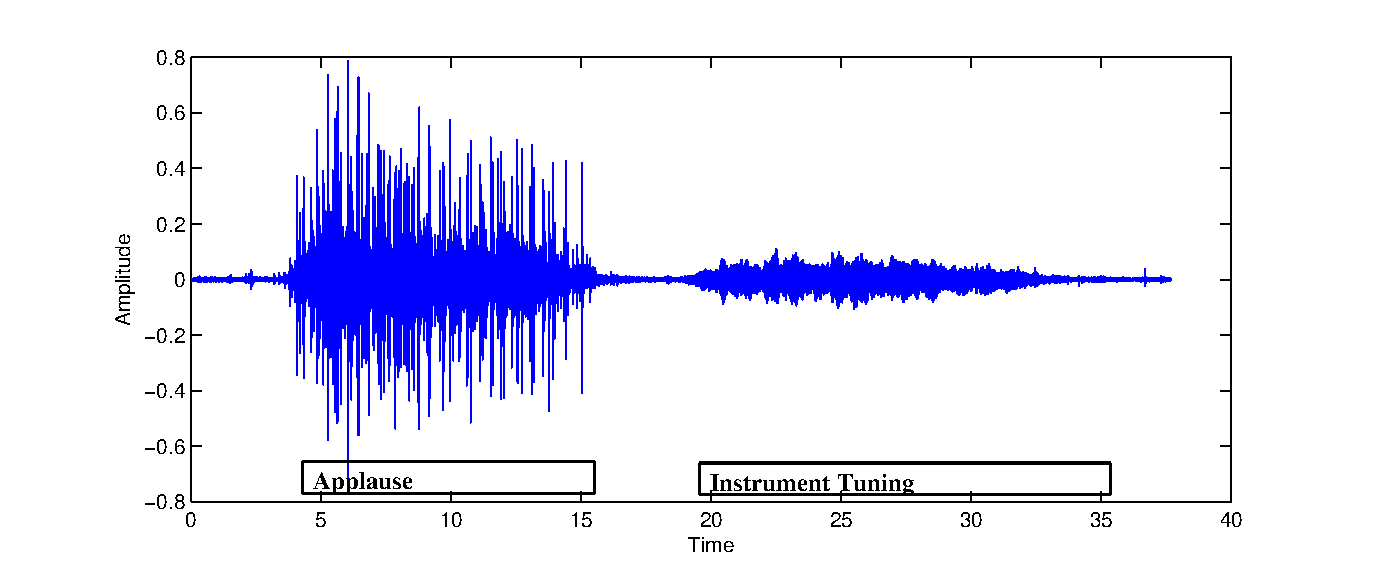
\includegraphics[scale=0.6]{figure/intro/waveform}
\caption{Waveform for a concert audio clip}
\label{fig:waveform}
\end{figure}

Figure \ref{fig:waveform} shows an example waveform for a concert environment. 
In this clip, two things happened. 
The first part of this waveform represents the sound when people are applauding. 
The second part is the sound when musicians are tuning their instruments. 
For a human, upon hearing these two things, we are easily to tell that this audio is recorded in a concert. 
And our problem throughout this thesis is to automatically detect out the events like \textit{applause} and \textit{instrument tuning}, 
and then to infer the scene \textit{concert} based on these two detected events. 

At here, we would like to give a detailed definition some terminology that we are going to use in this thesis. 

\section{Our Approach}
So in this thesis, we have proposed a system to automatically detect the events in an audio clip and then infer the scene or context from the detected audio events. 
We utilize a constructed audible event taxonomy, which helps us to categorize common audible events. 
Then Gaussian Mixture Models (GMMs) are built for modeling these audible events. 
We use audio data from Sound Search Engines where users can upload clips. 
The features we used for building GMMs are Mel-Frequency Cepstrum Coefficients (MFCCs). 
It is a popular feature for speech recognition, and we use it in our problem. 
In the scene recognition process, we first segment an audio clip by a segmenter, which uses frame energy and spectral centroid to calculate a threshold. 
After detecting for these segments, we use the relation we get from movie, play, TV series scripts to infer the scene of the original clip.  

\section{Thesis Organization}
The thesis is organizaed as follows: Chapter 2 gives a description about related works, in the area of audible events taxonomy, audio event detection and audio scene recognition. 
Chapter 3 reviews the data we used in this thesis, including event list and scene list. 
Then in chapter 4 we describes how event detection is carried out. 
Chapter 5 present the method we used to extract scene-event relations and scene recognition process. 
Evaluations of event detection and scene recognition are presented in chapter 6. 
Finally, chapter 7 gives a conclusion.   

